\section{Metodologia}

\frame
{
\frametitle{Cenário}
\begin{itemize}
	\item Equipe de três integrantes.
	\item Diferente disponibilidade de horários.
	\item Diferentes conjuntos de habilidades.
	\item Diferentes sistemas operacionais.
	\item Complexidade do projeto.
	\item \emph{Software} livre.
\end{itemize}
}

\subsection{Processo de Desenvolvimento do Software}
\frame
{
\frametitle{Processo de Desenvolvimento do Software}
\begin{itemize}
	\item Metodologia inspirada em Métodos Ágeis:
	\begin{itemize}
		\item \emph{Software} funcional.
		\item Documentação sucinta.
		\item Desenvolvimento orientado a testes.
	\end{itemize}
	\item Reuniões periódicas:
	\begin{itemize}
		\item Controle de qualidade.
		\item Revisão de código.
		\item Estabelecimento de novas metas.
		\item Alocação das tarefas.
	\end{itemize}
\end{itemize}
}
\frame
{
\frametitle{Desenvolvimento Orientado a Testes}
\begin{itemize}
	% TODO: substituir esse ciclo em texto por uma figura bacana como essa:
	% http://blog.fasagri.com.br/wp-content/uploads/2011/11/ciclo.png
	\item Ciclo original:
	\begin{enumerate}
		\item Adicionar teste.
		\item Executar testes e verificar falhas.
		\item Escrever código e corrigir falhas.
		\item Refatorar código.
		\item Repetir.
	\end{enumerate}
	\item Adaptação do ciclo.
	\item Vantagens:
	\begin{itemize}
		\item Passos menores.
		\item Cumprimento de metas.
		\item Minimiza os \emph{bugs}.
		\item Mantém a simplicidade do código.
	\end{itemize}
\end{itemize}
}
\frame
{
\frametitle{Revisão de Código}
\begin{itemize}
	\item Examinação sistemática do código-fonte.
	\item Processos classificados em:
	\begin{itemize}
		\item Programação em pares.
		\item Revisão de código formal.
		\item Revisão de código leve.
	\end{itemize}
	\item Revisão auxiliada por ferramenta.
\end{itemize}
}

\subsection{Ferramentas Utilizadas}
\frame
{
\frametitle{Ferramentas Utilizadas}
\begin{itemize}
	\item Sistema Gerenciador de Banco de Dados.
	\item Linguagens de Programação.
	\item Gerenciamento e Automação de Projetos.
	\item Sistema de Controle de Versão.
	\item Testes e Cobertura de Código.
\end{itemize}
}

\frame
{
\frametitle{Sistema Gerenciador de Banco de Dados}
\begin{itemize}
	\item Bancos de dados relacionais são inadequados para este caso.
	\item Solução: Bancos de dados de grafos.
\end{itemize}
\begin{table}[!htb]
	\centering
	\setlength{\tabcolsep}{2pt}
	\scriptsize
	\caption{Comparação entre as opções de SGBDs disponíveis}
	\newcolumntype{C}{c}
	\only<2->{\newcolumntype{C}{>{\columncolor{blue!10}}c}}
	\begin{tabular}{lccCc}
		\hline
		& \textbf{HyperGraphDB} & \textbf{InfoGrid} & \textbf{Neo4j} & \textbf{OrientDB} \\
		\hline
		\textbf{Licença} & LGPL & AGPLv3 & AGPLv3 & Apache \\
		\textbf{Iniciado em} & 2005 & ? & 2003 & ? \\
		\textbf{Versão estável} & 1.1 & 2.9.5 & 1.4.2 & 0.9.25 \\
		\textbf{Data versão estável} & Dezembro 2010 & Agosto 2011 & Setembro 2011 & Março 2011 \\
		\textbf{Bindings Java} & Sim & Sim & Sim & Sim \\
		\textbf{Bindings Python} & Não & Não & Sim & Parcial \\
		\textbf{Bindings C/C++} & Não & Não & Não & Não \\
		\textbf{Stand-alone} & Sim & ? & Sim & Sim \\
		\textbf{Embarcado} & Não & ? & Sim & Sim \\
		\textbf{Suporte Blueprints} & Não & Não & Sim & Sim \\
		\hline
	\end{tabular}
	\\ ~ \\
	\tiny
	Fonte: Autoria própria.
\end{table}
}

\frame
{
\frametitle{Linguagens de Programação}
\begin{itemize}
	\item No servidor:
	\begin{itemize}
		\item Alternativas consideradas:
		\begin{itemize}
			\item C++.
			\item Java.
			\item Python.
		\end{itemize}
		\item Decisão influenciada pelo SGBD (Neo4j).
		\item Linguagem escolhida: Java.
	\end{itemize}
	\item No cliente \emph{web}:
	\begin{itemize}
		\item Alternativas consideradas:
		\begin{itemize}
			\item Applets Java.
			\item JavaScript.
		\end{itemize}
		\item Linguagem escolhida: JavaScript.
	\end{itemize}
\end{itemize}
}

\frame
{
\frametitle{Gerenciamento e Automação de Projetos}
	\begin{itemize}
		\item O \emph{software} possui vários módulos (sub-projetos).
		\item O \emph{software} depende de várias bibliotecas.
		\item Necessidade de uma ferramenta capaz de:
		\begin{itemize}
			\item Facilitar o processo de \emph{build} e integração dos módulos.
			\item Simplificar a resolução de dependências.
			\item Executar os testes unitários e de integração.
			\item Facilitar o gerenciamento de projetos grandes.
		\end{itemize}
		\item Solução: Apache Maven.
	\end{itemize}
}

\frame
{
\frametitle{Sistema de Controle de Versão}
	\begin{itemize}
		\item Sistemas de Controle de Versão Centralizados.
		\item Sistemas de Controle de Versão Distribuídos.
		\item Vantagens dos Distribuídos:
		\begin{itemize}
			\item \emph{Merges} são mais fáceis.
			\item Não há necessidade de um repositório central.
			\item \emph{Commits} podem ser feitos mesmo sem acesso à Internet.
		\end{itemize}
		\item Sistema escolhido: git.
		\item Hospedagem do repositório no GitHub{\textsuperscript\textregistered}:
		\begin{itemize}
			\item Visibilidade do projeto.
			\item \emph{Issues}.
			\item \emph{Milestones}.
			\item \emph{Code review}.
		\end{itemize}
	\end{itemize}
}

\frame
{
\frametitle{Testes e Cobertura de Código}
\begin{figure}
	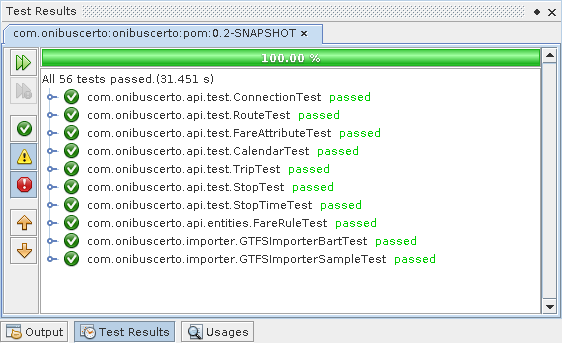
\includegraphics[width=0.85\textwidth]{./imgs/testes.png}
	\caption{JUnit}
	\tiny
	Fonte: Autoria própria.
\end{figure}
}

\frame
{
\frametitle{Testes e Cobertura de Código}
\begin{figure}
	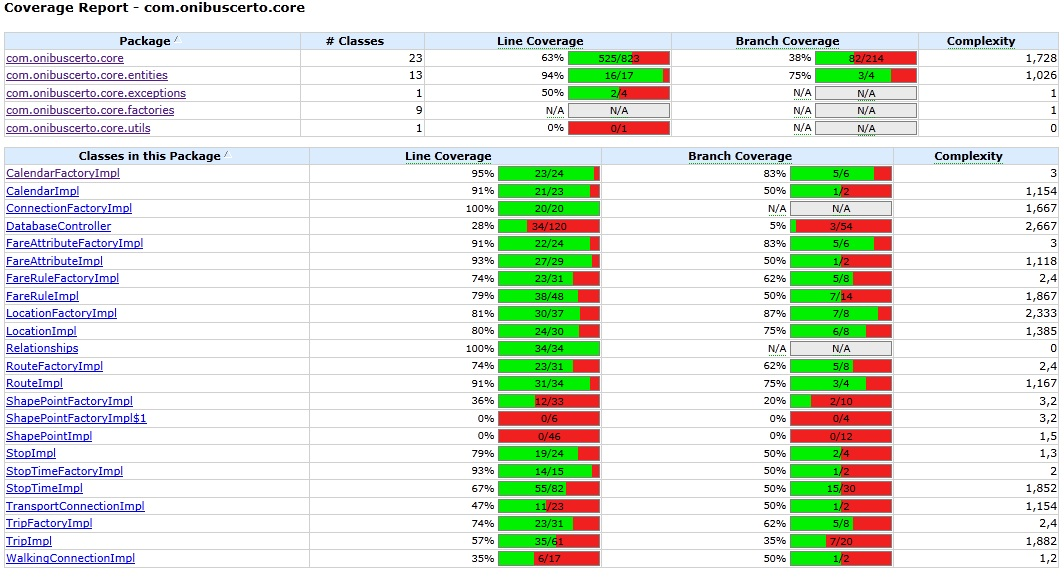
\includegraphics[width=\textwidth]{./imgs/cobertura.png}
	\caption{Cobertura}
	\tiny
	Fonte: Autoria própria.
\end{figure}
}
